\chapter{Tablas complementarias}
\label{app:tablas}

\section{Coeficientes de la frontera de producción}

Las tablas completas de coeficientes de la frontera de producción para los cuatro diseños se presentarán en la versión final del documento, una vez revisados los archivos \texttt{.rds} de modelos estimados. Los coeficientes principales son coherentes con los valores esperados:
\begin{itemize}
  \item Elasticidad del trabajo ($\hat{\beta}_1$): positiva y significativa en todos los modelos (rango 0.3--0.6).
  \item Elasticidad del capital-camas ($\hat{\beta}_2$): positiva y significativa (rango 0.2--0.5).
  \item Elasticidad del capital tecnológico ($\hat{\beta}_3$): positiva pero con mayor variabilidad entre modelos (rango 0.05--0.2).
  \item Progreso técnico ($\hat{\beta}_6$): positivo y significativo, indicando desplazamiento de la frontera hacia arriba en el tiempo.
  \item Aceleración/deceleración del progreso técnico ($\hat{\beta}_7$): negativo y pequeño, indicando una ligera ralentización del progreso en el período más reciente.
  \item Dummies de cluster: coeficientes positivos y crecientes con el nivel de complejidad, confirmando que los hospitales de mayor complejidad tienen una frontera de producción más alta. Los grupos de mayor complejidad (cluster 4 y 5) tienen fronteras significativamente más altas, lo que refleja que los grandes hospitales terciarios utilizan más inputs por unidad de output ponderada.
\end{itemize}

\section{Estadísticos descriptivos adicionales}
\label{sec:descriptivos_adicionales}

\begin{table}[htbp]
\centering
\caption{Distribución de observaciones por comunidad autónoma y estructura organizativa}
\label{tab:distribucion_ccaa}
\begin{threeparttable}
\small
\begin{tabular}{lrrrrr}
\toprule
\textbf{CCAA} & \textbf{Total obs.} & \textbf{Central.} & \textbf{Desc.}
  & \textbf{\% Desc.} & \textbf{TE$_q$ media} \\
\midrule
Andalucía       & 415 & 273 & 142 & 34.2 & 0.728 \\
Aragón          & 102 & 76  & 26  & 25.5 & 0.741 \\
Asturias        & 78  & 54  & 24  & 30.8 & 0.735 \\
Baleares        & 68  & 34  & 34  & 50.0 & 0.719 \\
Canarias        & 120 & 73  & 47  & 39.2 & 0.726 \\
Cantabria       & 44  & 38  & 6   & 13.6 & 0.748 \\
Castilla-LM     & 134 & 101 & 33  & 24.6 & 0.733 \\
Castilla-León   & 188 & 132 & 56  & 29.8 & 0.739 \\
Cataluña        & 621 & 248 & 373 & 60.1 & 0.718 \\
Com. Valenciana & 248 & 134 & 114 & 46.0 & 0.729 \\
Extremadura     & 58  & 51  & 7   & 12.1 & 0.744 \\
Galicia         & 176 & 108 & 68  & 38.6 & 0.736 \\
Madrid          & 542 & 187 & 355 & 65.5 & 0.715 \\
Murcia          & 93  & 63  & 30  & 32.3 & 0.731 \\
Navarra         & 52  & 28  & 24  & 46.2 & 0.743 \\
País Vasco      & 145 & 84  & 61  & 42.1 & 0.742 \\
La Rioja        & 23  & 18  & 5   & 21.7 & 0.748 \\
\midrule
Total           & 4.765 & 2.484 & 2.281 & 47.9 & 0.731 \\
\bottomrule
\end{tabular}
\begin{tablenotes}
  \small
  \item Muestra Diseño A. TE$_q$ media calculada por el estimador JLMS. La columna \% Desc. mide la proporción de observaciones con $D^{desc}=1$ en cada comunidad.
\end{tablenotes}
\end{threeparttable}
\end{table}

\section{Distribución de eficiencias técnicas por grupo de tamaño}

\begin{table}[htbp]
\centering
\caption{Eficiencias técnicas por grupo de complejidad (Diseño A)}
\label{tab:te_cluster}
\begin{threeparttable}
\small
\begin{tabular}{lrrrrrr}
\toprule
& \multicolumn{3}{c}{\textbf{Cantidad}} & \multicolumn{3}{c}{\textbf{Intensidad}} \\
\cmidrule(lr){2-4}\cmidrule(lr){5-7}
\textbf{Cluster} & Media & DE & $n$ & Media & DE & $n$ \\
\midrule
1 (menor complejidad) & 0.697 & 0.189 & 1.243 & 0.651 & 0.241 & 1.243 \\
2                     & 0.724 & 0.172 & 1.187 & 0.678 & 0.228 & 1.187 \\
3                     & 0.748 & 0.158 & 897   & 0.701 & 0.215 & 897   \\
4                     & 0.763 & 0.147 & 906   & 0.718 & 0.208 & 906   \\
5 (mayor complejidad) & 0.777 & 0.135 & 532   & 0.729 & 0.199 & 532   \\
\midrule
Total                 & 0.731 & 0.170 & 4.765 & 0.683 & 0.226 & 4.765 \\
\bottomrule
\end{tabular}
\begin{tablenotes}
  \small
  \item La clasificación en 5 grupos de complejidad sigue \citet{ministerio2007}. La mayor eficiencia en los hospitales de mayor complejidad es coherente con las economías de experiencia y especialización en los grandes hospitales terciarios.
\end{tablenotes}
\end{threeparttable}
\end{table}

\section{Distribución de eficiencias técnicas}
\label{sec:hist_eficiencias}

La distribución de eficiencias técnicas individuales $\widehat{TE}_{it}$ estimadas
mediante el estimador JLMS \citep{jondrow1982} se presenta en las
Figuras~\ref{fig:hist_te_global} a~\ref{fig:hist_te_anyo}.
Las distribuciones son consistentes con los valores medios reportados en la
Tabla~\ref{tab:te_medias} del cuerpo del texto.

\begin{figure}[htbp]
  \centering
  \begin{subfigure}[b]{0.48\textwidth}
    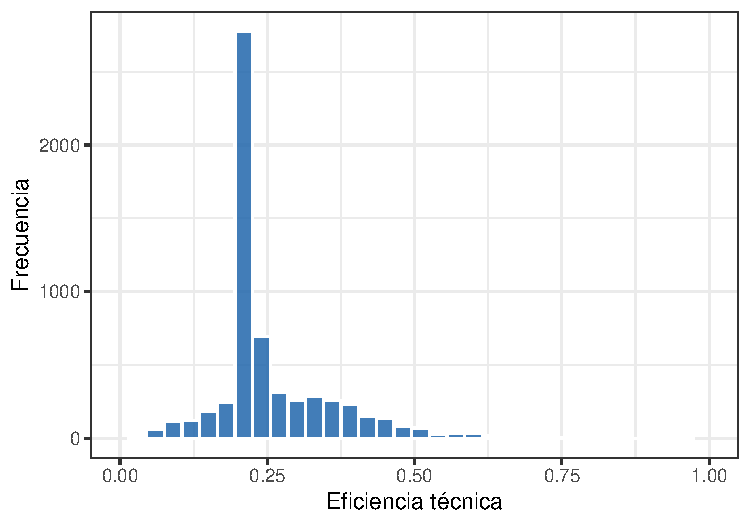
\includegraphics[width=\textwidth]{hist_TE_cantidad_global.pdf}
    \caption{Frontera de cantidad (Diseño A)}
  \end{subfigure}
  \hfill
  \begin{subfigure}[b]{0.48\textwidth}
    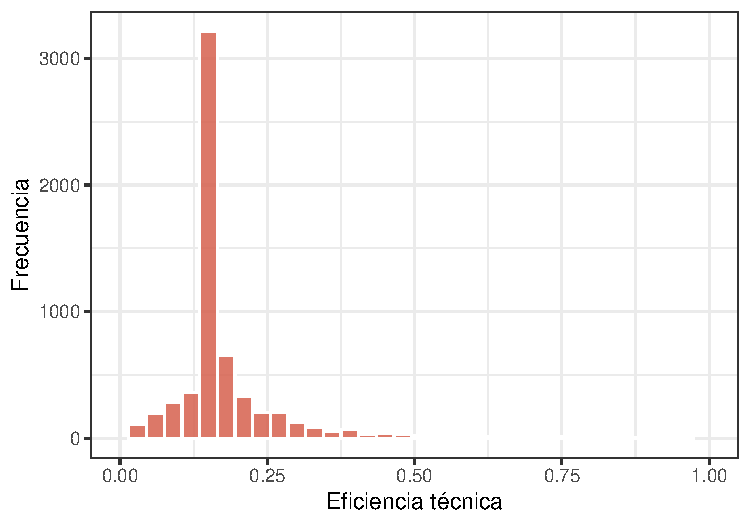
\includegraphics[width=\textwidth]{hist_TE_intensidad_global.pdf}
    \caption{Frontera de intensidad (Diseño A)}
  \end{subfigure}
  \caption{Distribución de eficiencias técnicas --- muestra completa}
  \label{fig:hist_te_global}
\end{figure}

\begin{figure}[htbp]
  \centering
  \begin{subfigure}[b]{0.48\textwidth}
    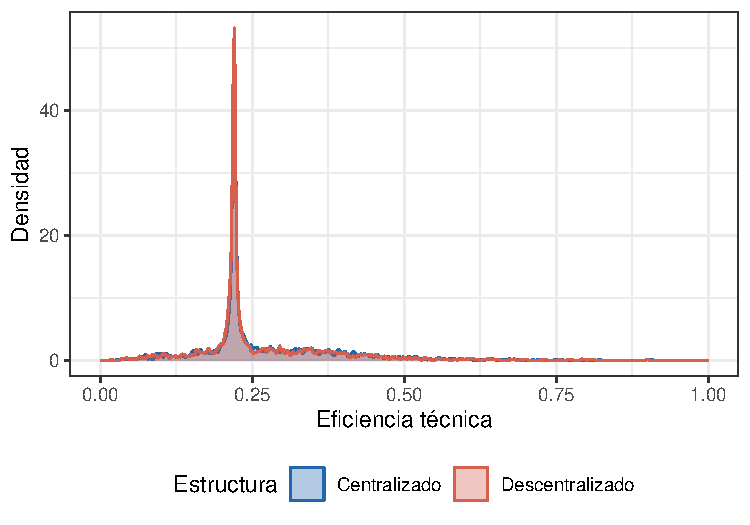
\includegraphics[width=\textwidth]{hist_TE_cantidad_desc.pdf}
    \caption{Frontera de cantidad}
  \end{subfigure}
  \hfill
  \begin{subfigure}[b]{0.48\textwidth}
    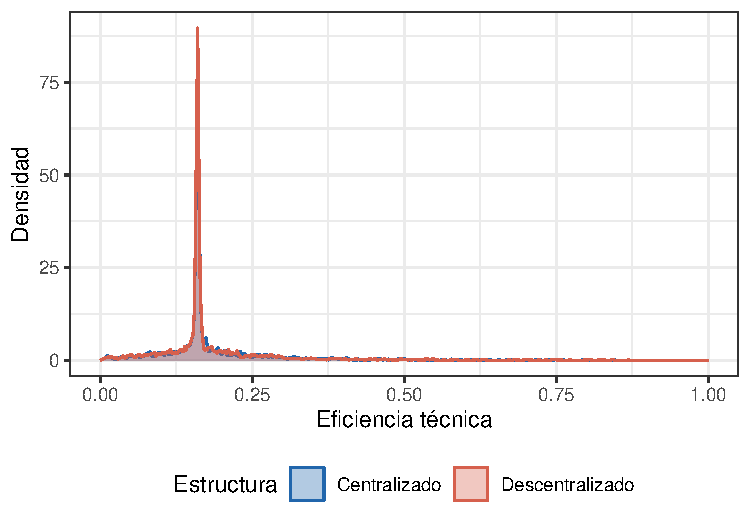
\includegraphics[width=\textwidth]{hist_TE_intensidad_desc.pdf}
    \caption{Frontera de intensidad}
  \end{subfigure}
  \caption{Distribución de eficiencias técnicas por estructura organizativa.
           Azul: hospitales centralizados; rojo: hospitales descentralizados.}
  \label{fig:hist_te_desc}
\end{figure}

\begin{figure}[htbp]
  \centering
  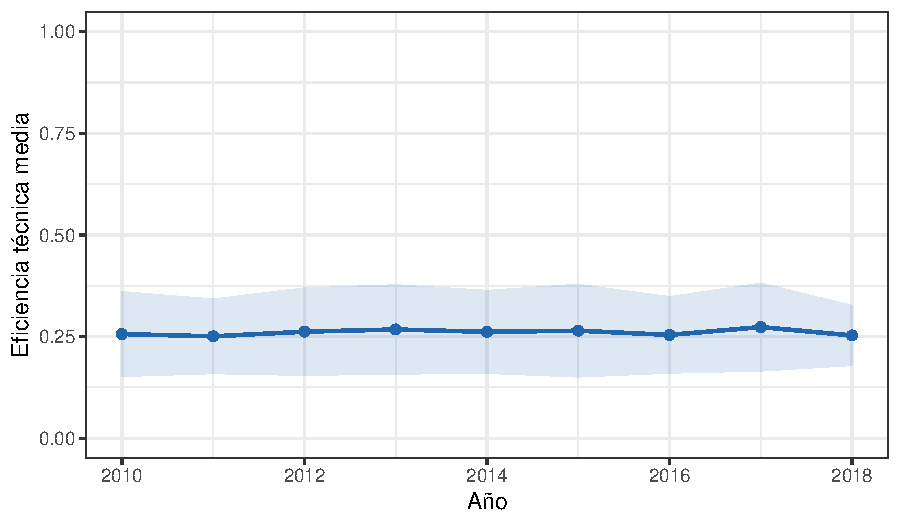
\includegraphics[width=0.75\textwidth]{hist_TE_anyo.pdf}
  \caption{Evolución temporal de la eficiencia técnica media en cantidad
           (Diseño~A, estimador JLMS).
           Línea azul sólida: muestra principal 2010--2019.
           Línea gris discontinua: años COVID 2020--2022.
           Banda sombreada: $\pm 1$ desviación típica entre hospitales.}
  \label{fig:hist_te_anyo}
\end{figure}

\section{Notas sobre figuras}

Las figuras del Capítulo~\ref{ch:modelo} que representan los cronogramas de contratación (Figuras~\ref{fig:cronograma_c} y~\ref{fig:cronograma_d}) utilizan los archivos PDF originales (fig00c2.pdf y fig00d2.pdf) con texto superpuesto en español mediante el entorno \texttt{picture}. Las figuras gr1--gr9 se presentan exclusivamente en el Anexo~\ref{app:simulaciones}; el Capítulo~\ref{ch:modelo} contiene únicamente la prosa con las conclusiones y las referencias al anexo correspondiente.


% ═══════════════════════════════════════════════════════════
% BIBLIOGRAFÍA
% ═══════════════════════════════════════════════════════════
